\documentclass[11pt,a4paper,oneside]{report}

% --- Korean and fonts ---
\usepackage[hangul]{kotex}
\setmainhangulfont{Malgun Gothic}
\setsanshangulfont{Malgun Gothic}
\setmonohangulfont{Malgun Gothic}

% --- Layout ---
\usepackage[a4paper,margin=2.25cm,top=2.45cm,bottom=2.45cm]{geometry}
\usepackage{setspace}
\linespread{1.13}
\setlength{\parskip}{0.35em}
\setlength{\parindent}{0pt}

% --- Tables, lists, graphics ---
\usepackage{amsmath,amssymb}
\usepackage{booktabs,tabularx,longtable,array}
\usepackage{enumitem}
\usepackage{graphicx}
\usepackage{xcolor}
\usepackage{tikz}
\usetikzlibrary{arrows.meta,positioning,fit}

% --- Boxes ---
\usepackage[most]{tcolorbox}
\newtcolorbox{infobox}[1][]{colback=blue!4,colframe=blue!45!black,sharp corners,boxrule=0.5pt,#1}
\newtcolorbox{warnbox}[1][]{colback=red!4,colframe=red!45!black,sharp corners,boxrule=0.5pt,#1}
\newtcolorbox{checkbox}[1][]{colback=green!4,colframe=green!45!black,sharp corners,boxrule=0.5pt,#1}

% --- Code listings ---
\usepackage{listings}
\definecolor{codebg}{RGB}{248,248,245}
\definecolor{coderule}{RGB}{210,210,210}
\definecolor{codecomment}{RGB}{85,130,65}
\definecolor{codekw}{RGB}{20,70,160}
\lstdefinestyle{base}{
  basicstyle=\ttfamily\footnotesize,
  backgroundcolor=\color{codebg},
  frame=single,
  rulecolor=\color{coderule},
  showstringspaces=false,
  breaklines=true,
  breakatwhitespace=false,
  columns=fullflexible,
  keepspaces=true,
  tabsize=2,
  captionpos=b
}
\lstdefinestyle{shell}{style=base}
\lstdefinestyle{yaml}{style=base,commentstyle=\color{codecomment},morecomment=[l]{\#}}
\lstdefinestyle{python}{style=base,language=Python,keywordstyle=\color{codekw}\bfseries,commentstyle=\color{codecomment}}
\lstset{style=base}

% --- Hyperlinks ---
\usepackage[colorlinks=true,linkcolor=blue!45!black,urlcolor=blue!55!black,citecolor=blue!45!black]{hyperref}
\usepackage{url}

\title{\textbf{LC-EKF VIO 제로베이스 구축 매뉴얼}\\[0.35em]
\large ROS 없이 C++20, OpenCV, Eigen, yaml-cpp로 빌드하고 실행하기}
\author{\texttt{D:/02\_research/04\_cpp\_LC-EKF\_VIO}}
\date{2026-05-01}

\begin{document}
\maketitle

\begin{abstract}
이 문서는 \texttt{D:/02\_research/04\_cpp\_LC-EKF\_VIO} 폴더의 LC-EKF VIO 시스템을
빈 Windows/WSL 환경에서 다시 구축하기 위한 절차서다. 대상 독자는 저장소를 처음 받은
사람이며, 목표는 의존성 설치, 데이터 배치, YAML 설정, CMake 빌드, 단일 실행,
결과 검증까지 재현 가능한 상태로 만드는 것이다. 본 시스템은 ROS, catkin, colcon 없이
순수 CMake 기반으로 동작한다.
\end{abstract}

\tableofcontents
\clearpage

% =====================================================================
\chapter{매뉴얼 범위}
% =====================================================================

\section{목표 산출물}

제로베이스 구축이 끝나면 다음 상태가 되어야 한다.

\begin{longtable}{p{0.25\textwidth}p{0.68\textwidth}}
\toprule
항목 & 완료 기준 \\
\midrule
빌드 산출물 & \texttt{build/run\_vio}, \texttt{build/run\_euroc} 실행 파일 생성 \\
설정 파일 & \texttt{config/*.yaml}의 \texttt{dataset}, \texttt{output}, \texttt{T\_cam\_imu}가 현재 환경과 일치 \\
데이터셋 & KITTI raw 또는 EuRoC 디렉터리가 reader가 기대하는 구조로 배치 \\
실행 결과 & \texttt{results/<run\_name>/trajectory\_tum.txt}, \texttt{metrics.txt}, \texttt{state\_log.txt} 생성 \\
시각화 & \texttt{trajectory\_plot.png}, \texttt{state\_plot.png} 생성 \\
\bottomrule
\end{longtable}

\begin{infobox}
\textbf{기준 환경}: 이 프로젝트의 표준 빌드 경로는 WSL Ubuntu이다. Windows 네이티브 빌드도
이론상 가능하지만 OpenCV, Eigen, yaml-cpp 설치 방식이 환경마다 달라 재현성이 낮다.
따라서 본 매뉴얼은 Windows 파일시스템에 저장소를 두고 WSL에서 빌드하는 방식을 기준으로 한다.
\end{infobox}

\section{시스템 구성}

\begin{center}
\resizebox{\textwidth}{!}{%
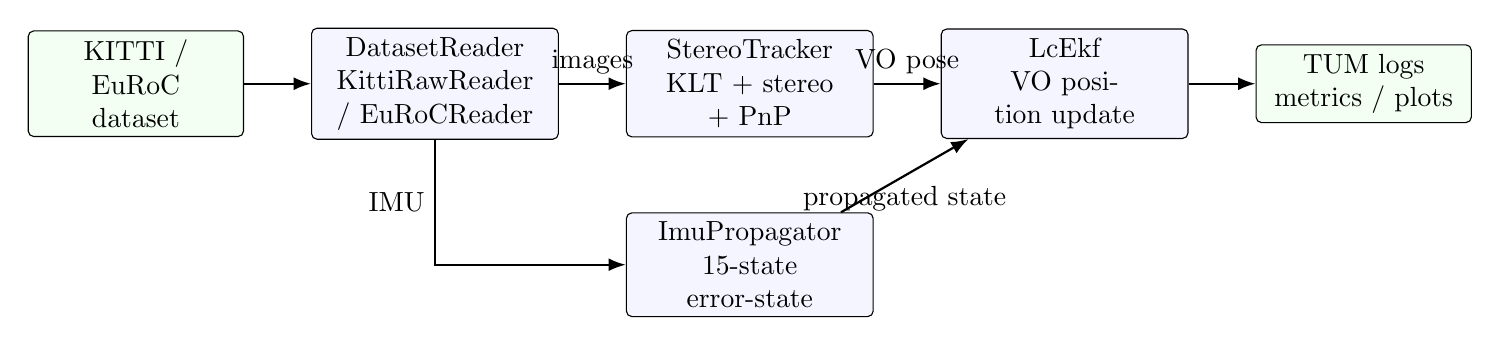
\begin{tikzpicture}[
  node distance=0.95cm and 0.85cm,
  box/.style={draw,rounded corners=2pt,minimum height=0.9cm,text width=2.9cm,align=center,fill=blue!4},
  io/.style={draw,rounded corners=2pt,minimum height=0.9cm,text width=2.5cm,align=center,fill=green!5},
  arr/.style={-{Latex[length=2.2mm]},thick}
]
\node[io] (data) {KITTI / EuRoC\\dataset};
\node[box,right=of data] (reader) {DatasetReader\\KittiRawReader / EuRoCReader};
\node[box,right=of reader] (tracker) {StereoTracker\\KLT + stereo + PnP};
\node[box,below=of tracker] (imu) {ImuPropagator\\15-state error-state};
\node[box,right=of tracker] (ekf) {LcEkf\\VO position update};
\node[io,right=of ekf] (out) {TUM logs\\metrics / plots};

\draw[arr] (data) -- (reader);
\draw[arr] (reader) -- node[above]{images} (tracker);
\draw[arr] (reader) |- node[pos=0.25,left]{IMU} (imu);
\draw[arr] (tracker) -- node[above]{VO pose} (ekf);
\draw[arr] (imu) -- node[below]{propagated state} (ekf);
\draw[arr] (ekf) -- (out);
\end{tikzpicture}
}
\end{center}

핵심 타깃은 \texttt{run\_vio} 하나다. \texttt{dataset\_type}이 \texttt{euroc}이면
EuRoC reader를, \texttt{kitti\_raw}이면 KITTI raw reader를 사용한다.

% =====================================================================
\chapter{수학적 방법론}
% =====================================================================

\section{좌표계와 변환 convention}

이 프로젝트의 수식은 코드의 변수명과 맞추어 쓴다. \(W\)는 world frame,
\(I\)는 IMU/body frame, \(C\)는 cam0 frame이다. 회전 \(R_{AB}\)는
\(B\) frame 벡터를 \(A\) frame으로 보낸다.

\begin{center}
\resizebox{0.95\textwidth}{!}{%
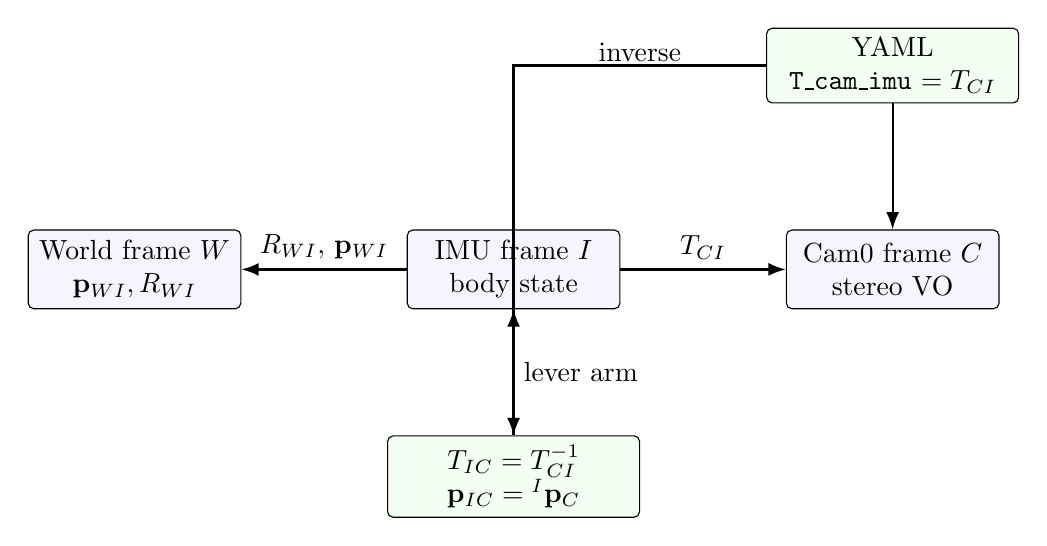
\begin{tikzpicture}[
  node distance=1.6cm and 2.1cm,
  framebox/.style={draw,rounded corners=2pt,minimum width=2.7cm,minimum height=1.0cm,align=center,fill=blue!4},
  calbox/.style={draw,rounded corners=2pt,minimum width=3.2cm,minimum height=0.9cm,align=center,fill=green!5},
  arr/.style={-{Latex[length=2.2mm]},thick}
]
\node[framebox] (W) {World frame \(W\)\\\(\mathbf{p}_{WI}, R_{WI}\)};
\node[framebox,right=of W] (I) {IMU frame \(I\)\\body state};
\node[framebox,right=of I] (C) {Cam0 frame \(C\)\\stereo VO};

\node[calbox,below=of I] (tic) {\(T_{IC}=T_{CI}^{-1}\)\\\(\mathbf{p}_{IC}={}^{I}\mathbf{p}_C\)};
\node[calbox,above=of C] (tci) {YAML\\\texttt{T\_cam\_imu} \(=T_{CI}\)};

\draw[arr] (I) -- node[above]{\(R_{WI},\,\mathbf{p}_{WI}\)} (W);
\draw[arr] (I) -- node[above]{\(T_{CI}\)} (C);
\draw[arr] (tci) -- (C);
\draw[arr] (tci.west) -| node[pos=0.25,above,fill=white,inner sep=1pt]{inverse} (tic.north);
\draw[arr] (tic) -- node[right]{lever arm} (I);
\end{tikzpicture}
}
\smallskip

\small\textbf{그림 2.1:} 코드와 YAML이 사용하는 좌표계. EKF 상태는 \(W\leftarrow I\),
YAML calibration은 \(C\leftarrow I\), update lever arm은 \(I\leftarrow C\)를 사용한다.
\end{center}

\begin{equation}
{}^{A}\mathbf{p}
= R_{AB}\,{}^{B}\mathbf{p} + {}^{A}\mathbf{p}_{B}.
\end{equation}

YAML의 \texttt{T\_cam\_imu}는 \(T_{CI}\), 즉 IMU 좌표계의 점을 camera 좌표계로
보내는 변환이다. LC-EKF 업데이트에서는 cam0 origin의 IMU 좌표가 필요하므로
\(T_{IC}=T_{CI}^{-1}\)를 사용하고,

\begin{equation}
\mathbf{p}_{IC} = {}^{I}\mathbf{p}_{C}
= \left(T_{IC}\right)_{0:3,3}
\end{equation}

를 lever arm으로 둔다. 코드에서는 \texttt{LcEkf} 생성자에서 이 값을 계산한다.

\begin{longtable}{p{0.22\textwidth}p{0.68\textwidth}}
\toprule
기호 & 의미 \\
\midrule
\(\mathbf{p}_{WI}\) & world frame에서 본 IMU 위치 \\
\(\mathbf{v}_{WI}\) & world frame에서 본 IMU 속도 \\
\(R_{WI}\) & IMU 벡터를 world 벡터로 보내는 자세 \\
\(\mathbf{b}_g,\mathbf{b}_a\) & gyro/accel bias \\
\(\mathbf{p}_{IC}\) & IMU frame에서 본 cam0 origin 위치 \\
\(\mathbf{z}_{VO}\) & stereo VO가 제공하는 cam0 위치 측정값 \\
\bottomrule
\end{longtable}

\section{상태와 오차 상태}

공칭 상태는 위치, 속도, 자세, bias로 구성된다.

\begin{equation}
\mathbf{x}
= \left\{
\mathbf{p}_{WI},\,
\mathbf{v}_{WI},\,
R_{WI},\,
\mathbf{b}_g,\,
\mathbf{b}_a
\right\}.
\end{equation}

EKF 공분산은 회전 행렬 자체가 아니라 작은 회전 오차 \(\delta\boldsymbol{\theta}\)를
포함하는 15차원 error-state에 대해 유지한다.

\begin{equation}
\delta\mathbf{x}
=
\begin{bmatrix}
\delta\mathbf{p}^{\top} &
\delta\mathbf{v}^{\top} &
\delta\boldsymbol{\theta}^{\top} &
\delta\mathbf{b}_g^{\top} &
\delta\mathbf{b}_a^{\top}
\end{bmatrix}^{\top}
\in \mathbb{R}^{15}.
\end{equation}

자세 보정은 SO(3)의 exponential map으로 적용한다.

\begin{equation}
R_{WI} \leftarrow R_{WI}\operatorname{Exp}(\delta\boldsymbol{\theta}).
\end{equation}

\begin{center}
\resizebox{\textwidth}{!}{%
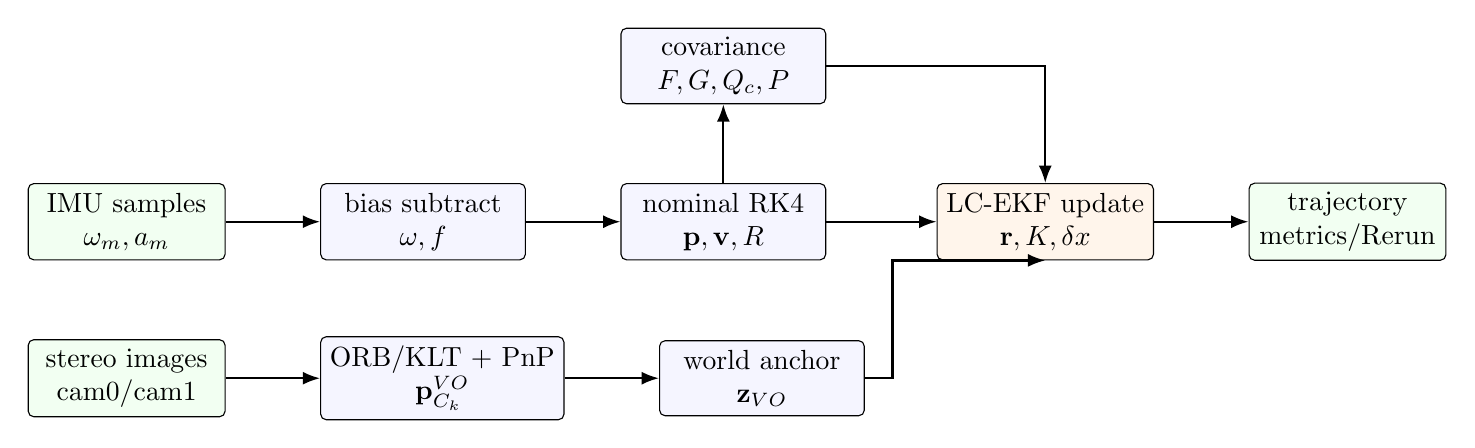
\begin{tikzpicture}[
  node distance=1.0cm and 1.2cm,
  box/.style={draw,rounded corners=2pt,minimum width=2.6cm,minimum height=0.85cm,align=center,fill=blue!4},
  iobox/.style={draw,rounded corners=2pt,minimum width=2.5cm,minimum height=0.85cm,align=center,fill=green!5},
  warn/.style={draw,rounded corners=2pt,minimum width=2.7cm,minimum height=0.85cm,align=center,fill=orange!8},
  arr/.style={-{Latex[length=2.2mm]},thick}
]
\node[iobox] (imu) {IMU samples\\\(\omega_m,a_m\)};
\node[box,right=of imu] (bias) {bias subtract\\\(\omega,f\)};
\node[box,right=of bias] (rk4) {nominal RK4\\\(\mathbf{p},\mathbf{v},R\)};
\node[box,above=of rk4] (cov) {covariance\\\(F,G,Q_c,P\)};

\node[iobox,below=of imu] (img) {stereo images\\cam0/cam1};
\node[box,right=of img] (vo) {ORB/KLT + PnP\\\(\mathbf{p}^{VO}_{C_k}\)};
\node[box,right=of vo] (anchor) {world anchor\\\(\mathbf{z}_{VO}\)};

\node[warn,right=1.4cm of rk4] (ekf) {LC-EKF update\\\(\mathbf{r},K,\delta x\)};
\node[iobox,right=of ekf] (out) {trajectory\\metrics/Rerun};

\draw[arr] (imu) -- (bias);
\draw[arr] (bias) -- (rk4);
\draw[arr] (rk4.north) -- (cov.south);
\draw[arr] (rk4) -- (ekf);
\draw[arr] (cov.east) -| (ekf.north);
\draw[arr] (img) -- (vo);
\draw[arr] (vo) -- (anchor);
\draw[arr] (anchor.east) -- ++(0.35,0) |- (ekf.south);
\draw[arr] (ekf) -- (out);
\end{tikzpicture}
}
\smallskip

\small\textbf{그림 2.2:} 수학적 처리 흐름. IMU는 예측을 만들고, stereo VO는 cam0 위치
측정값을 만들며, LC-EKF는 두 정보를 위치 update로 결합한다.
\end{center}

\section{IMU 측정 모델과 공칭 상태 전파}

gyro와 accelerometer raw 측정값을 다음처럼 둔다.

\begin{align}
\boldsymbol{\omega}
&= \boldsymbol{\omega}_m - \mathbf{b}_g - \mathbf{n}_g, \\
\mathbf{f}
&= \mathbf{a}_m - \mathbf{b}_a - \mathbf{n}_a.
\end{align}

여기서 \(\mathbf{f}\)는 IMU frame의 specific force이다. 공칭 상태 동역학은 다음이다.

\begin{align}
\dot{\mathbf{p}}_{WI} &= \mathbf{v}_{WI}, \\
\dot{\mathbf{v}}_{WI} &= R_{WI}\mathbf{f} + \mathbf{g}_{W}, \\
\dot{R}_{WI} &= R_{WI}\,[\boldsymbol{\omega}]_{\times}, \\
\dot{\mathbf{b}}_g &= \mathbf{0}, \\
\dot{\mathbf{b}}_a &= \mathbf{0}.
\end{align}

구현에서는 bias를 뺀 \(\boldsymbol{\omega}\), \(\mathbf{f}\)를 사용해 위치와 속도를 RK4로
적분하고, 자세는

\begin{equation}
R_{k+1} = R_k\operatorname{Exp}(\Delta t\,\boldsymbol{\omega})
\end{equation}

로 갱신한 뒤 quaternion normalization으로 다시 정규직교화한다.

\section{초기 정렬}

초기화는 GT를 쓰지 않고 첫 카메라 timestamp 이후
\texttt{init.static\_window\_sec} 구간의 IMU 평균으로 수행한다.

\begin{align}
\bar{\boldsymbol{\omega}} &=
\frac{1}{N}\sum_{i=1}^{N}\boldsymbol{\omega}_{m,i}, \\
\bar{\mathbf{a}} &=
\frac{1}{N}\sum_{i=1}^{N}\mathbf{a}_{m,i}.
\end{align}

초기 gyro bias는 \(\mathbf{b}_{g,0}=\bar{\boldsymbol{\omega}}\)로 둔다.
초기 자세는 정지 상태에서

\begin{equation}
R_{WI,0}\bar{\mathbf{a}} \approx
\begin{bmatrix}0&0&g\end{bmatrix}^{\top},
\qquad
\mathbf{g}_{W} =
\begin{bmatrix}0&0&-g\end{bmatrix}^{\top}
\end{equation}

가 되도록 \(\bar{\mathbf{a}}\)를 world \(+Z\) 방향에 맞춘다. 이 조건이면 정지 상태에서
\(R_{WI}\mathbf{f}+\mathbf{g}_W \approx \mathbf{0}\)이 된다.

\section{15-state 공분산 전파}

오차 상태의 연속시간 근사는 다음 꼴이다.

\begin{equation}
\delta\dot{\mathbf{x}} = F\delta\mathbf{x} + G\mathbf{n},
\qquad
\mathbf{n} =
\begin{bmatrix}
\mathbf{n}_g^{\top} &
\mathbf{n}_a^{\top} &
\mathbf{n}_{wg}^{\top} &
\mathbf{n}_{wa}^{\top}
\end{bmatrix}^{\top}.
\end{equation}

구현에서 사용하는 주요 \(F\) block은 다음이다.

\begin{align}
F_{p,v} &= I, \\
F_{v,\theta} &= -R_{WI}[\mathbf{f}]_{\times}, &
F_{v,b_a} &= -R_{WI}, \\
F_{\theta,\theta} &= -[\boldsymbol{\omega}]_{\times}, &
F_{\theta,b_g} &= -R_{WI}.
\end{align}

noise injection \(G\)는 accel noise가 속도 오차로, gyro noise가 자세 오차로,
bias random walk가 각각 bias 오차로 들어가도록 구성한다.

\begin{align}
G_{v,n_a} &= R_{WI}, &
G_{\theta,n_g} &= R_{WI}, \\
G_{b_g,n_{wg}} &= I, &
G_{b_a,n_{wa}} &= I.
\end{align}

연속 noise density는 YAML의 \texttt{imu\_noise} 값으로 만든다.

\begin{equation}
Q_c =
\operatorname{diag}
\left(
\sigma_g^2 I,\,
\sigma_a^2 I,\,
\sigma_{bg}^2 I,\,
\sigma_{ba}^2 I
\right).
\end{equation}

이산화는 1차 Euler 근사다.

\begin{align}
\Phi &\approx I + F\Delta t, \\
P_{k+1} &= \Phi P_k \Phi^{\top}
        + GQ_cG^{\top}\Delta t.
\end{align}

따라서 공칭 상태는 RK4로 비교적 정교하게 적분하지만, 공분산은 단순 1차 근사로 전파한다.

\section{Stereo VO 측정과 world anchoring}

Stereo VO는 첫 cam0 frame을 local world로 두고 상대 camera pose를 추정한다.
초기 frame에서는 rectified stereo pair에서 ORB matching을 수행하고, disparity로 깊이를 얻는다.

\begin{align}
Z &= \frac{f_x b}{d}, \\
X &= \frac{(u-c_x)Z}{f_x}, \\
Y &= \frac{(v-c_y)Z}{f_y}.
\end{align}

이후 frame에서는 좌측 이미지 KLT tracking으로 2D-3D 대응을 유지하고,
PnP RANSAC으로 camera pose를 구한다.

\begin{equation}
\min_{R,t}
\sum_i
\rho\left(
\left\|
\pi\left(K(R\mathbf{P}_i+t)\right)-\mathbf{u}_i
\right\|^2
\right).
\end{equation}

VO local 좌표계의 camera 위치 \(\mathbf{p}^{VO}_{C_k}\)는 첫 cam0 pose를 기준으로
EKF world에 anchor된다.

\begin{align}
R_{WC_0} &= R_{WI,0}R_{IC}, \\
\mathbf{p}_{WC_0} &= R_{WI,0}\mathbf{p}_{IC} + \mathbf{p}_{WI,0}, \\
\mathbf{p}^{W}_{C_k} &= R_{WC_0}\mathbf{p}^{VO}_{C_k} + \mathbf{p}_{WC_0}.
\end{align}

이 \(\mathbf{p}^{W}_{C_k}\)가 LC-EKF의 위치 측정값으로 들어간다.

\section{LC-EKF 위치 업데이트}

측정값은 world frame에서 본 cam0 origin 위치다.

\begin{equation}
\mathbf{z}_{VO} = \mathbf{p}^{W}_{C}.
\end{equation}

현재 EKF 상태로 예측한 cam0 위치는 IMU 위치와 lever arm으로 계산한다.

\begin{equation}
h(\mathbf{x})
= \mathbf{p}_{WI} + R_{WI}\mathbf{p}_{IC}.
\end{equation}

innovation은

\begin{equation}
\mathbf{r} = \mathbf{z}_{VO} - h(\mathbf{x})
\end{equation}

이고, 측정 Jacobian의 non-zero block은 다음 두 개다.

\begin{align}
H_p &= I, \\
H_{\theta} &= -R_{WI}[\mathbf{p}_{IC}]_{\times}.
\end{align}

VO 측정 noise는 scalar 설정 \(\sigma_{VO}\)로부터

\begin{equation}
R_{VO} = \sigma_{VO}^{2}I
\end{equation}

로 둔다. Kalman update는 표준식과 Joseph form 공분산 갱신을 사용한다.

\begin{center}
\resizebox{0.98\textwidth}{!}{%
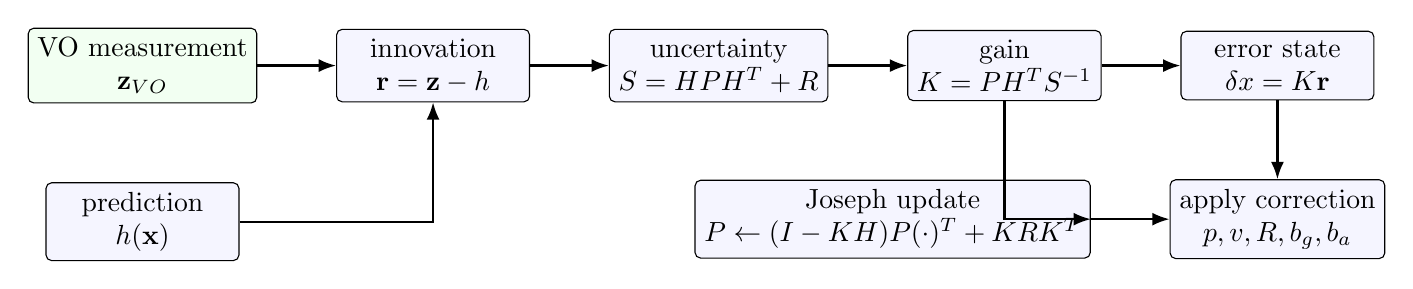
\begin{tikzpicture}[
  node distance=1.0cm and 1.0cm,
  box/.style={draw,rounded corners=2pt,minimum width=2.45cm,minimum height=0.82cm,align=center,fill=blue!4},
  meas/.style={draw,rounded corners=2pt,minimum width=2.45cm,minimum height=0.82cm,align=center,fill=green!5},
  arr/.style={-{Latex[length=2.2mm]},thick}
]
\node[meas] (z) {VO measurement\\\(\mathbf{z}_{VO}\)};
\node[box,below=of z] (h) {prediction\\\(h(\mathbf{x})\)};
\node[box,right=of z] (r) {innovation\\\(\mathbf{r}=\mathbf{z}-h\)};
\node[box,right=of r] (s) {uncertainty\\\(S=HPH^T+R\)};
\node[box,right=of s] (k) {gain\\\(K=PH^TS^{-1}\)};
\node[box,right=of k] (dx) {error state\\\(\delta x=K\mathbf{r}\)};
\node[box,below=of dx] (apply) {apply correction\\\(p,v,R,b_g,b_a\)};
\node[box,left=of apply] (p) {Joseph update\\\(P\leftarrow(I-KH)P(\cdot)^T+KRK^T\)};

\draw[arr] (z) -- (r);
\draw[arr] (h) -| (r);
\draw[arr] (r) -- (s);
\draw[arr] (s) -- (k);
\draw[arr] (k) -- (dx);
\draw[arr] (dx) -- (apply);
\draw[arr] (k) |- (p);
\draw[arr] (p) -- (apply);
\end{tikzpicture}
}
\smallskip

\small\textbf{그림 2.3:} LC-EKF 위치 업데이트 내부 흐름. 측정 residual로 error-state를
계산한 뒤 공칭 상태와 공분산을 함께 보정한다.
\end{center}

\begin{align}
S &= HPH^{\top}+R_{VO}, \\
K &= PH^{\top}S^{-1}, \\
\delta\mathbf{x} &= K\mathbf{r}, \\
P &\leftarrow (I-KH)P(I-KH)^{\top}+KR_{VO}K^{\top}.
\end{align}

상태 보정은 다음처럼 적용한다.

\begin{align}
\mathbf{p} &\leftarrow \mathbf{p}+\delta\mathbf{p}, \\
\mathbf{v} &\leftarrow \mathbf{v}+\delta\mathbf{v}, \\
R &\leftarrow R\operatorname{Exp}(\delta\boldsymbol{\theta}), \\
\mathbf{b}_g &\leftarrow \mathbf{b}_g+\delta\mathbf{b}_g, \\
\mathbf{b}_a &\leftarrow \mathbf{b}_a+\delta\mathbf{b}_a.
\end{align}

\begin{infobox}
이 구조가 \textbf{loose coupling}인 이유는 raw feature residual을 EKF가 직접 쓰지 않고,
frontend가 이미 계산한 VO camera 위치만 측정값으로 쓰기 때문이다. 구현은 단순하지만
VO outlier나 scale/depth 오류가 위치 측정값에 그대로 들어올 수 있다.
\end{infobox}

\section{IMU-only 설정의 의미}

\texttt{config/euroc\_v202\_imuonly.yaml}은 별도의 전파-only 실행기를 쓰는 것이 아니라
\(\sigma_{VO}=10^9\)로 설정한다. 따라서

\begin{equation}
R_{VO}=\sigma_{VO}^{2}I
\end{equation}

가 매우 커지고,

\begin{equation}
K = PH^{\top}(HPH^{\top}+R_{VO})^{-1} \approx 0
\end{equation}

가 된다. 결과적으로 VO update가 실행되더라도 EKF 상태 보정량은 거의 0이므로,
trajectory는 IMU propagation에 의해 지배된다.

\section{ATE RMSE 계산}

결과 검증의 ATE는 추정 위치열 \(\mathbf{p}^{est}_i\)와 GT 위치열
\(\mathbf{p}^{gt}_i\) 사이의 rigid alignment를 먼저 구한 뒤 계산한다.
코드는 Eigen의 \texttt{umeyama(..., false)}를 사용하므로 scale은 고정하고
회전과 평행이동만 맞춘다.

\begin{equation}
T^{*}
= \arg\min_{T\in SE(3)}
\sum_{i}
\left\|
T\mathbf{p}^{est}_i - \mathbf{p}^{gt}_i
\right\|^{2}.
\end{equation}

ATE RMSE는 다음이다.

\begin{equation}
\operatorname{ATE}_{RMSE}
=
\sqrt{
\frac{1}{N}
\sum_{i=1}^{N}
\left\|
T^{*}\mathbf{p}^{est}_i - \mathbf{p}^{gt}_i
\right\|^{2}
}.
\end{equation}

따라서 \texttt{metrics.txt}의 ATE는 절대 좌표 원점 차이보다 trajectory 모양과 누적 오차를
비교하는 지표에 가깝다.

% =====================================================================
\chapter{사전 준비}
% =====================================================================

\section{Windows와 WSL}

Windows PowerShell에서 WSL Ubuntu가 있는지 확인한다.

\begin{lstlisting}[style=shell,caption={PowerShell에서 WSL 확인}]
wsl -l -v
\end{lstlisting}

Ubuntu가 없다면 Microsoft Store 또는 관리자 PowerShell에서 WSL2 Ubuntu를 설치한다.
설치 후 Ubuntu 터미널을 열고 다음부터는 WSL 셸에서 작업한다.

\begin{lstlisting}[style=shell,caption={WSL에서 저장소 위치로 이동}]
cd /mnt/d/02_research/04_cpp_LC-EKF_VIO
pwd
\end{lstlisting}

\begin{warnbox}
YAML 설정에는 Windows 경로 \texttt{D:\textbackslash ...}를 넣지 않는다. WSL에서 실행할 때는
\texttt{/mnt/d/...} 또는 저장소 루트 기준 상대 경로를 사용한다.
\end{warnbox}

\section{시스템 패키지 설치}

처음 세팅하는 Ubuntu에서 다음 패키지를 설치한다.

\begin{lstlisting}[style=shell,caption={필수 빌드 및 실행 의존성}]
sudo apt update
sudo apt install -y \
  build-essential cmake git pkg-config unzip \
  libeigen3-dev libopencv-dev libyaml-cpp-dev \
  python3 python3-numpy python3-matplotlib
\end{lstlisting}

버전 확인:

\begin{lstlisting}[style=shell,caption={도구 버전 확인}]
g++ --version
cmake --version
pkg-config --modversion opencv4
python3 - <<'PY'
import numpy, matplotlib
print("numpy", numpy.__version__)
print("matplotlib", matplotlib.__version__)
PY
\end{lstlisting}

\section{저장소 구조 확인}

소스 폴더가 정상이라면 루트에 다음 항목이 있어야 한다.

\begin{lstlisting}[style=shell,caption={루트 구조}]
apps/        # run_vio.cpp
config/      # dataset and calibration YAML
docs/        # manuals and generated PDF
include/     # public headers
src/         # implementation
tools/       # plot_trajectory.py
CMakeLists.txt
README.md
\end{lstlisting}

이 프로젝트는 \texttt{build/}, \texttt{build\_rerun/}, \texttt{results/}, \texttt{logs/} 같은
생성물을 포함할 수 있다. 제로베이스 환경에서는 없어도 된다.

% =====================================================================
\chapter{데이터셋 배치}
% =====================================================================

\section{KITTI raw}

KITTI raw를 사용할 때 reader가 기대하는 최소 구조는 다음과 같다.

\begin{lstlisting}[style=shell,caption={KITTI raw 권장 배치}]
data/kitti_raw/
└── 2011_09_26/
    ├── calib_cam_to_cam.txt
    ├── calib_imu_to_velo.txt
    ├── calib_velo_to_cam.txt
    └── 2011_09_26_drive_0117_sync/
        ├── image_00/
        │   ├── data/*.png
        │   └── timestamps.txt
        ├── image_01/
        │   ├── data/*.png
        │   └── timestamps.txt
        └── oxts/
            ├── data/*.txt
            ├── timestamps.txt
            └── dataformat.txt
\end{lstlisting}

흑백 스테레오 폴더는 \texttt{image\_00}/\texttt{image\_01}이다. reader는 우선 이 쌍을
찾고, 없을 때만 컬러 페어인 \texttt{image\_02}/\texttt{image\_03}을 찾는다. OXTS는
IMU와 ground truth 계산에 사용된다.

\begin{checkbox}
\textbf{KITTI 체크리스트}
\begin{itemize}[leftmargin=1.4em]
\item 날짜 디렉터리 바로 아래에 calib 3종이 있는가.
\item drive 디렉터리 이름이 \texttt{*\_sync}로 끝나는가.
\item \texttt{image\_00/data}와 \texttt{image\_01/data}에 같은 개수의 PNG가 있는가.
\item \texttt{oxts/data/*.txt}와 \texttt{oxts/timestamps.txt}가 있는가.
\end{itemize}
\end{checkbox}

\section{EuRoC}

EuRoC reader는 root 바로 아래에 다음 폴더가 있다고 가정한다.

\begin{lstlisting}[style=shell,caption={EuRoC reader가 기대하는 구조}]
<dataset_root>/
├── imu0/data.csv
├── cam0/data.csv
├── cam0/data/*.png
├── cam1/data.csv
├── cam1/data/*.png
└── state_groundtruth_estimate0/data.csv
\end{lstlisting}

공식 EuRoC ASL 압축을 풀면 보통 \texttt{MH\_01\_easy/mav0/...} 형태가 된다.
그 경우 YAML의 \texttt{dataset}은 \texttt{MH\_01\_easy}가 아니라 \texttt{MH\_01\_easy/mav0}
까지 지정해야 한다.

% =====================================================================
\chapter{YAML 설정}
% =====================================================================

\section{경로 정책}

제로베이스에서 가장 흔한 실패는 오래된 절대 경로다. 현재 저장소에 포함된 일부 KITTI
설정은 과거 루트인 \texttt{/mnt/d/02\_research/06\_cpp\_LC-EKF\_VIO\_kitti\_raw}를
가리킬 수 있다. 이 문서의 대상 루트는 다음이다.

\begin{lstlisting}[style=shell]
/mnt/d/02_research/04_cpp_LC-EKF_VIO
\end{lstlisting}

저장소 루트에서 실행한다면 상대 경로가 가장 덜 깨진다.

\begin{lstlisting}[style=yaml,caption={권장 경로 설정}]
dataset_type: "kitti_raw"
dataset: "data/kitti_raw/2011_09_26/2011_09_26_drive_0117_sync"
output:  "results/kitti_raw_2011_09_26_drive_0117"
max_frames: 0
\end{lstlisting}

만약 \texttt{cd build} 안에서 실행한다면 상대 경로 기준이 바뀌므로 다음 중 하나를 선택한다.

\begin{itemize}[leftmargin=1.4em]
\item 저장소 루트에서만 실행한다: \texttt{./build/run\_vio config/...yaml}
\item YAML 경로를 절대 WSL 경로로 쓴다: \texttt{/mnt/d/02\_research/04\_cpp\_LC-EKF\_VIO/...}
\item build 디렉터리 기준 상대 경로로 바꾼다: \texttt{../data/...}, \texttt{../results/...}
\end{itemize}

\section{필수 키}

\begin{longtable}{p{0.30\textwidth}p{0.60\textwidth}}
\toprule
키 & 의미 \\
\midrule
\texttt{dataset\_type} & \texttt{euroc} 또는 \texttt{kitti\_raw} \\
\texttt{dataset} & reader가 읽을 데이터셋 root \\
\texttt{output} & 로그와 trajectory 파일을 저장할 디렉터리 \\
\texttt{max\_frames} & 0이면 전체, 양수면 해당 프레임 수까지만 실행 \\
\texttt{init.static\_window\_sec} & 초기 IMU 정지구간 평균 시간 \\
\texttt{imu\_noise} & gyro/accel white noise와 random walk \\
\texttt{ekf.sigma\_vo} & VO 위치 측정 잡음. 작을수록 VO를 더 신뢰 \\
\texttt{cam0}, \texttt{cam1} & intrinsics, distortion, \texttt{T\_cam\_imu} \\
\bottomrule
\end{longtable}

\section{KITTI 캘리브레이션 추출}

KITTI raw의 calib 3종에서 이 프로젝트가 요구하는 것은 rectified cam0/cam1 기준
\texttt{T\_cam\_imu} 두 개다. 의미는 \textbf{IMU 좌표계의 점을 camera 좌표계로 보내는}
\(T_{CI}\)이다.

\begin{align*}
T_{\text{cam0,imu}} &= R_{\text{rect,00}} \, T_{\text{cam,velo}} \, T_{\text{velo,imu}} \\
T_{\text{cam1,imu}} &= T_{\text{cam1,cam0}} \, T_{\text{cam0,imu}}
\end{align*}

다음 스크립트를 임시 파일로 저장해 실행하면 intrinsics와 두 행렬을 확인할 수 있다.

\begin{lstlisting}[style=python,caption={KITTI calib에서 YAML 값 추출}]
from pathlib import Path
import numpy as np

CALIB = Path("/mnt/d/02_research/04_cpp_LC-EKF_VIO/data/kitti_raw/2011_09_26")

def parse_kv(path):
    out = {}
    for line in path.read_text().splitlines():
        if ":" not in line:
            continue
        k, v = line.split(":", 1)
        out[k.strip()] = np.fromstring(v, sep=" ")
    return out

def homog(R, t):
    T = np.eye(4)
    T[:3, :3] = R.reshape(3, 3)
    T[:3, 3] = t.reshape(3)
    return T

cam = parse_kv(CALIB / "calib_cam_to_cam.txt")
v2c = parse_kv(CALIB / "calib_velo_to_cam.txt")
i2v = parse_kv(CALIB / "calib_imu_to_velo.txt")

T_cam_velo = homog(v2c["R"], v2c["T"])
T_velo_imu = homog(i2v["R"], i2v["T"])
R_rect_00 = np.eye(4)
R_rect_00[:3, :3] = cam["R_rect_00"].reshape(3, 3)

T_cam0_imu = R_rect_00 @ T_cam_velo @ T_velo_imu

P_rect_00 = cam["P_rect_00"].reshape(3, 4)
P_rect_01 = cam["P_rect_01"].reshape(3, 4)
fx, fy = P_rect_00[0, 0], P_rect_00[1, 1]
cx, cy = P_rect_00[0, 2], P_rect_00[1, 2]
baseline_x = -P_rect_01[0, 3] / fx

T_cam1_cam0 = np.eye(4)
T_cam1_cam0[0, 3] = -baseline_x
T_cam1_imu = T_cam1_cam0 @ T_cam0_imu

print(f"width height: {cam['S_rect_00'][0]:.0f} {cam['S_rect_00'][1]:.0f}")
print(f"fx fy cx cy: {fx:.4f} {fy:.4f} {cx:.4f} {cy:.4f}")
print(f"baseline_x: {baseline_x:.6f}")
for name, T in [("cam0", T_cam0_imu), ("cam1", T_cam1_imu)]:
    print(name)
    for row in T:
        print("  - [" + ", ".join(f"{v: .12f}" for v in row) + " ]")
\end{lstlisting}

\begin{warnbox}
KITTI rectified 이미지를 기준으로 쓸 때 왜곡 계수 \texttt{k1}, \texttt{k2}, \texttt{p1},
\texttt{p2}는 보통 0으로 둔다. \texttt{R\_rect\_00} 적용을 빠뜨리면 intrinsics와 좌표계가
어긋나 trajectory가 크게 발산한다.
\end{warnbox}

\section{최소 KITTI YAML 예시}

\begin{lstlisting}[style=yaml,caption={저장소 루트 실행 기준 최소 예시}]
dataset_type: "kitti_raw"
dataset: "data/kitti_raw/2011_09_26/2011_09_26_drive_0117_sync"
output:  "results/kitti_raw_2011_09_26_drive_0117"
max_frames: 0

init:
  mode: "stationary_imu"
  static_window_sec: 1.0
  gravity_norm: 9.81

imu_noise:
  gyro:       1.6968e-4
  accel:      2.0000e-3
  gyro_walk:  1.9393e-5
  accel_walk: 3.0000e-3

ekf:
  sigma_vo: 0.10

cam0:
  width: 1242
  height: 375
  fx: 721.5377
  fy: 721.5377
  cx: 609.5593
  cy: 172.8540
  k1: 0.0
  k2: 0.0
  p1: 0.0
  p2: 0.0
  T_cam_imu:
    - [ 0.000998747206, -0.999990382071,  0.004259378488, -0.314076869806 ]
    - [ 0.008416901828, -0.004250821136, -0.999955569675,  0.719452035633 ]
    - [ 0.999964048697,  0.001034553284,  0.008412575209, -1.089082940192 ]
    - [ 0.0,             0.0,             0.0,              1.0             ]

cam1:
  width: 1242
  height: 375
  fx: 721.5377
  fy: 721.5377
  cx: 609.5593
  cy: 172.8540
  k1: 0.0
  k2: 0.0
  p1: 0.0
  p2: 0.0
  T_cam_imu:
    - [ 0.000998748817, -0.999990390387,  0.004259383056, -0.851244549356 ]
    - [ 0.008416901410, -0.004250823329, -0.999955516666,  0.719451996647 ]
    - [ 0.999964103141,  0.001034555313,  0.008412574849, -1.089083003993 ]
    - [ 0.0,             0.0,             0.0,              1.0             ]
\end{lstlisting}

% =====================================================================
\chapter{빌드}
% =====================================================================

\section{일반 빌드}

WSL에서 저장소 루트로 이동한 뒤 configure와 build를 분리해 실행한다.

\begin{lstlisting}[style=shell,caption={Release 빌드}]
cd /mnt/d/02_research/04_cpp_LC-EKF_VIO
cmake -S . -B build -DCMAKE_BUILD_TYPE=Release
cmake --build build -j"$(nproc)"
\end{lstlisting}

성공하면 다음 파일이 생긴다.

\begin{lstlisting}[style=shell]
build/run_vio
build/run_euroc
\end{lstlisting}

\texttt{run\_euroc}는 과거 명령 호환용 이름이며 내부적으로 \texttt{apps/run\_vio.cpp}와
같은 main을 사용한다.

\section{Rerun 선택 빌드}

Rerun은 선택 기능이다. 일반 빌드는 Rerun SDK 없이 동작한다. Rerun 기록을 만들고 싶을 때만
별도 build 디렉터리를 사용한다.

\begin{lstlisting}[style=shell,caption={Rerun 활성 빌드}]
cd /mnt/d/02_research/04_cpp_LC-EKF_VIO
cmake -S . -B build_rerun -DCMAKE_BUILD_TYPE=Release -DENABLE_RERUN=ON
cmake --build build_rerun -j"$(nproc)"
\end{lstlisting}

\begin{warnbox}
\texttt{ENABLE\_RERUN=ON}은 CMake \texttt{FetchContent}로 Rerun C++ SDK zip을 내려받는다.
네트워크가 막힌 환경에서는 일반 빌드로 먼저 검증한 뒤, 사내/학교 네트워크 정책에 맞춰
SDK 캐시를 준비한다.
\end{warnbox}

\section{빌드 실패 빠른 판별}

\begin{longtable}{p{0.31\textwidth}p{0.58\textwidth}}
\toprule
증상 & 조치 \\
\midrule
\texttt{Eigen3Config.cmake not found} & \texttt{sudo apt install libeigen3-dev} \\
\texttt{OpenCVConfig.cmake not found} & \texttt{sudo apt install libopencv-dev} 후 \texttt{pkg-config --modversion opencv4} 확인 \\
\texttt{yaml-cpp not found} & \texttt{sudo apt install libyaml-cpp-dev} \\
\texttt{CMAKE\_CXX\_STANDARD 20} 관련 오류 & Ubuntu의 \texttt{g++}가 너무 오래됨. Ubuntu 22.04 이상 권장 \\
Rerun 다운로드 실패 & \texttt{-DENABLE\_RERUN=OFF} 일반 빌드로 우선 진행 \\
\bottomrule
\end{longtable}

% =====================================================================
\chapter{실행}
% =====================================================================

\section{단일 KITTI 실행}

항상 저장소 루트에서 실행하는 방식을 권장한다.

\begin{lstlisting}[style=shell,caption={KITTI 실행}]
cd /mnt/d/02_research/04_cpp_LC-EKF_VIO
./build/run_vio config/kitti_raw_2011_09_26_drive_0117.yaml
\end{lstlisting}

실행 마지막에 다음 형태가 나오면 정상이다.

\begin{lstlisting}[style=shell,caption={정상 종료 예시}]
========================================
Frames processed : 660
ATE RMSE         : 152.955 cm
Output           : results/kitti_raw_2011_09_26_drive_0117
========================================
\end{lstlisting}

이 저장소의 기존 결과 기준으로 \texttt{drive\_0001}은 108 frames, ATE 약 156 cm,
\texttt{drive\_0117}은 660 frames, ATE 약 153 cm 수준이다. LC-EKF 구조상 cm급 정밀도보다
미터급 누적 오차가 자연스럽다.

\section{단일 EuRoC 실행}

EuRoC는 YAML의 \texttt{dataset} 경로가 실제 \texttt{mav0} 구조를 가리키는지 먼저 확인한다.

\begin{lstlisting}[style=shell,caption={EuRoC 실행}]
cd /mnt/d/02_research/04_cpp_LC-EKF_VIO
./build/run_vio config/euroc_v101.yaml
\end{lstlisting}

\section{프레임 수 제한 테스트}

처음 환경 검증만 할 때는 YAML의 \texttt{max\_frames}를 50 또는 100으로 바꿔 빠르게
확인한다. 전체 실행 전 다음 항목만 보면 된다.

\begin{itemize}[leftmargin=1.4em]
\item \texttt{No camera data loaded}, \texttt{No IMU data loaded}가 없는가.
\item \texttt{tracked=} 값이 대부분 0이 아닌가.
\item \texttt{metrics.txt}가 생성되는가.
\end{itemize}

\section{Rerun 기록 생성}

Rerun 빌드를 사용하면 실행 결과를 \texttt{.rrd}로 저장할 수 있다.

\begin{lstlisting}[style=shell,caption={Rerun 파일 저장 실행}]
cd /mnt/d/02_research/04_cpp_LC-EKF_VIO
./build_rerun/run_vio \
  config/kitti_raw_2011_09_26_drive_0117.yaml \
  --rerun-save results/kitti_raw_2011_09_26_drive_0117/vio_rerun.rrd \
  --rerun-image-every 10
\end{lstlisting}

\texttt{--rerun-image-every 0}은 이미지 로깅을 끈다. 궤적과 scalar metric만 보고 싶으면
파일 크기를 크게 줄일 수 있다.

% =====================================================================
\chapter{결과 검증과 시각화}
% =====================================================================

\section{출력 파일}

\begin{longtable}{p{0.34\textwidth}p{0.56\textwidth}}
\toprule
파일 & 의미 \\
\midrule
\texttt{trajectory\_tum.txt} & EKF 추정 위치. TUM 형식 \\
\texttt{gt\_tum.txt} & ground truth 위치. GT가 있을 때만 생성 \\
\texttt{trajectory\_aligned\_tum.txt} & GT에 SE(3) 정렬한 추정 궤적 \\
\texttt{state\_log.txt} & position, velocity, Euler, quaternion, feature count \\
\texttt{imu\_log.txt} & 사용한 gyro/accel 로그 \\
\texttt{metrics.txt} & frames, ATE RMSE \\
\texttt{vio\_rerun.rrd} & Rerun 선택 실행 시 생성되는 기록 파일 \\
\bottomrule
\end{longtable}

\section{plot 생성}

Python 시각화 도구는 결과 디렉터리를 인자로 받는다.

\begin{lstlisting}[style=shell,caption={trajectory/state plot 생성}]
cd /mnt/d/02_research/04_cpp_LC-EKF_VIO
python3 tools/plot_trajectory.py results/kitti_raw_2011_09_26_drive_0117
\end{lstlisting}

생성물:

\begin{lstlisting}[style=shell]
results/kitti_raw_2011_09_26_drive_0117/trajectory_plot.png
results/kitti_raw_2011_09_26_drive_0117/state_plot.png
\end{lstlisting}

\section{정상/비정상 판정}

\begin{longtable}{p{0.26\textwidth}p{0.63\textwidth}}
\toprule
관찰값 & 판단 \\
\midrule
ATE 1--3 m, trajectory 모양이 GT와 유사 & KITTI 짧은 시퀀스 기준 정상 범위 \\
feature count가 초반부터 0 근처 & 이미지 경로, rectification, stereo baseline, 조명/텍스처 문제 확인 \\
ATE 10 m 이상 또는 한 방향으로 급발산 & \texttt{T\_cam\_imu} 행렬 순서, baseline 부호, dataset/output 경로 혼동 확인 \\
속도가 비현실적으로 커짐 & IMU timestamp 순서, gravity 방향, 초기 정지구간 확인 \\
GT unavailable & EuRoC ground truth 또는 KITTI OXTS 파일 누락 가능 \\
\bottomrule
\end{longtable}

% =====================================================================
\chapter{운영 절차 체크리스트}
% =====================================================================

\section{처음 구축할 때}

\begin{checkbox}
\begin{enumerate}[leftmargin=1.5em]
\item WSL Ubuntu에서 \texttt{g++}, \texttt{cmake}, OpenCV4, Eigen3, yaml-cpp 설치.
\item 저장소 루트가 \texttt{/mnt/d/02\_research/04\_cpp\_LC-EKF\_VIO}인지 확인.
\item KITTI 또는 EuRoC 데이터를 reader 구조에 맞게 배치.
\item YAML의 \texttt{dataset}과 \texttt{output}을 현재 경로로 수정.
\item KITTI라면 calib 3종에서 \texttt{T\_cam\_imu}와 intrinsics 확인.
\item \texttt{cmake -S . -B build -DCMAKE\_BUILD\_TYPE=Release} 실행.
\item \texttt{cmake --build build -j"\$(nproc)"} 실행.
\item \texttt{./build/run\_vio config/<run>.yaml} 실행.
\item \texttt{python3 tools/plot\_trajectory.py <result\_dir>} 실행.
\item \texttt{metrics.txt}, \texttt{trajectory\_plot.png}, \texttt{state\_plot.png} 확인.
\end{enumerate}
\end{checkbox}

\section{새 KITTI drive를 추가할 때}

\begin{enumerate}[leftmargin=1.5em]
\item 같은 날짜의 calib 파일이 이미 있으면 재사용한다.
\item 새 \texttt{*\_sync} drive 디렉터리만 날짜 폴더 아래에 추가한다.
\item 기존 YAML을 복사해 \texttt{dataset}, \texttt{output}, 필요 시 \texttt{max\_frames}만 바꾼다.
\item 날짜가 바뀌면 calib 추출을 다시 수행한다.
\item 짧은 \texttt{max\_frames: 100}으로 먼저 실행한 뒤 전체 프레임으로 돌린다.
\end{enumerate}

\section{새 개발자가 가장 먼저 볼 파일}

\begin{longtable}{p{0.32\textwidth}p{0.58\textwidth}}
\toprule
파일 & 이유 \\
\midrule
\texttt{CMakeLists.txt} & 의존성, 라이브러리, 실행 파일 타깃 정의 \\
\texttt{apps/run\_vio.cpp} & CLI, YAML 로딩, reader 선택, 메인 루프, 로그 저장 \\
\texttt{include/core/types.hpp} & 데이터 구조와 camera/IMU 파라미터 정의 \\
\texttt{include/io/*.hpp} & dataset reader가 기대하는 디렉터리 구조 \\
\texttt{include/frontend/stereo\_tracker.hpp} & stereo VO의 외부 인터페이스 \\
\texttt{include/ekf/*.hpp} & IMU propagation과 LC-EKF update 인터페이스 \\
\texttt{tools/plot\_trajectory.py} & 결과 파일 형식과 시각화 기준 \\
\bottomrule
\end{longtable}

% =====================================================================
\chapter{트러블슈팅}
% =====================================================================

\section{실행 전 오류}

\begin{longtable}{p{0.35\textwidth}p{0.54\textwidth}}
\toprule
오류 메시지 또는 증상 & 해결 방향 \\
\midrule
\texttt{Fatal: bad file} 또는 YAML 로딩 실패 & config 경로가 틀렸거나 YAML 문법 오류. 들여쓰기와 콜론 확인 \\
\texttt{Cannot find KITTI stereo image folders} & \texttt{dataset}이 drive root가 아니거나 \texttt{image\_00/data} 누락 \\
\texttt{No KITTI OXTS packets found} & \texttt{oxts/data/*.txt} 누락 또는 dataset 경로가 한 단계 어긋남 \\
\texttt{No camera data loaded} & EuRoC/KITTI root 구조가 reader 기대 구조와 다름 \\
\texttt{Camera config is missing a 4x4 T\_cam\_imu} & \texttt{cam0} 또는 \texttt{cam1} YAML 행렬 누락/행 개수 오류 \\
\bottomrule
\end{longtable}

\section{실행 후 성능 문제}

\begin{longtable}{p{0.31\textwidth}p{0.59\textwidth}}
\toprule
증상 & 확인할 것 \\
\midrule
프레임은 처리되지만 ATE가 매우 큼 & \texttt{T\_cam\_imu}가 \(T_{CI}\)인지, 역행렬 \(T_{IC}\)를 넣지 않았는지 확인 \\
좌우 feature가 거의 잡히지 않음 & cam0/cam1 경로가 바뀌었거나 baseline 부호가 반대일 수 있음 \\
초기부터 자세가 이상함 & \texttt{init.static\_window\_sec} 동안 실제로 정지에 가까운지 확인 \\
plot 스크립트가 import 오류 & \texttt{python3-numpy}, \texttt{python3-matplotlib} 설치 확인 \\
결과 디렉터리가 엉뚱한 곳에 생김 & YAML 상대 경로가 현재 작업 디렉터리 기준으로 해석됨 \\
\bottomrule
\end{longtable}

\section{경로 문제를 빠르게 찾는 명령}

\begin{lstlisting}[style=shell,caption={YAML 경로 대상 존재 여부 확인}]
cd /mnt/d/02_research/04_cpp_LC-EKF_VIO
python3 - <<'PY'
from pathlib import Path
import yaml

cfg_path = Path("config/kitti_raw_2011_09_26_drive_0117.yaml")
cfg = yaml.safe_load(cfg_path.read_text())
root = Path(cfg["dataset"])
print("dataset:", root, "exists=", root.exists())
for p in ["image_00/data", "image_01/data", "oxts/data"]:
    q = root / p
    print(p, q.exists(), len(list(q.glob("*"))) if q.exists() else 0)
print("output:", Path(cfg["output"]))
PY
\end{lstlisting}

\begin{warnbox}
위 진단 명령은 PyYAML이 설치되어 있을 때만 동작한다. 설치되어 있지 않다면
\texttt{sudo apt install python3-yaml}을 사용하거나 YAML 파일을 직접 열어 경로를 확인한다.
\end{warnbox}

% =====================================================================
\chapter{부록: 한 번에 따라 하는 명령}
% =====================================================================

\section{EuRoC V2\_02 빠른 실행}

PowerShell에서 WSL 명령을 한 줄로 실행하려면 다음 형태를 사용한다. 저장소 루트는
\texttt{/mnt/d/02\_research/04\_cpp\_LC-EKF\_VIO}이다.

\begin{lstlisting}[style=shell,caption={일반 빌드와 EuRoC V2\_02 실행}]
# Normal build
wsl bash -lc 'cd /mnt/d/02_research/04_cpp_LC-EKF_VIO && cmake --build build -j$(nproc)'

# Run EuRoC V2_02_medium
wsl bash -lc 'cd /mnt/d/02_research/04_cpp_LC-EKF_VIO && ./build/run_vio config/euroc_v202.yaml'
\end{lstlisting}

\begin{infobox}
현재 확인된 \texttt{euroc\_v202.yaml} 실행 기준 결과는 전체 \texttt{2348} 프레임 처리,
ATE RMSE 약 \texttt{58.98 cm}, 출력 폴더 \texttt{results/euroc\_v202}이다.
\end{infobox}

\section{EuRoC V2\_02 IMU-only 실행}

IMU-only 설정은 기존 KITTI 방식과 동일하게 \texttt{ekf.sigma\_vo}를 매우 크게 두어
VO 위치 보정 영향을 사실상 끄는 방식이다. 설정 파일은
\texttt{config/euroc\_v202\_imuonly.yaml}이고, 결과는
\texttt{results/euroc\_v202\_imuonly}에 저장된다.

\begin{lstlisting}[style=shell,caption={IMU-only 실행과 결과 확인}]
# Run IMU-only
wsl bash -lc 'cd /mnt/d/02_research/04_cpp_LC-EKF_VIO && ./build/run_vio config/euroc_v202_imuonly.yaml'

# Check metrics
wsl bash -lc 'cd /mnt/d/02_research/04_cpp_LC-EKF_VIO && cat results/euroc_v202_imuonly/metrics.txt'

# Compare normal VIO vs IMU-only
wsl bash -lc 'cd /mnt/d/02_research/04_cpp_LC-EKF_VIO && cat results/euroc_v202/metrics.txt && cat results/euroc_v202_imuonly/metrics.txt'
\end{lstlisting}

\begin{infobox}
\texttt{cat}은 Linux/WSL에서 파일 내용을 터미널에 출력하는 명령이다.
PowerShell의 \texttt{Get-Content}와 같은 용도로 사용한다.
\end{infobox}

\section{EuRoC V2\_02 Rerun 기록}

Rerun을 사용할 때 기존 \texttt{build\_rerun} 캐시가 예전 저장소 경로를 물고 있으면
새 빌드 폴더를 쓰는 편이 안전하다. 아래 예시는 \texttt{build\_rerun\_v202}를 사용한다.

\begin{lstlisting}[style=shell,caption={Rerun 빌드와 일반 VIO 기록}]
# Rerun build
wsl bash -lc 'cd /mnt/d/02_research/04_cpp_LC-EKF_VIO && cmake -S . -B build_rerun_v202 -DCMAKE_BUILD_TYPE=Release -DENABLE_RERUN=ON && cmake --build build_rerun_v202 -j$(nproc)'

# Record normal VIO
wsl bash -lc 'cd /mnt/d/02_research/04_cpp_LC-EKF_VIO && ./build_rerun_v202/run_vio config/euroc_v202.yaml --rerun-save results/euroc_v202/euroc_v202_unified_time.rrd --rerun-image-every 10'

# Open from PowerShell
rerun D:\02_research\04_cpp_LC-EKF_VIO\results\euroc_v202\euroc_v202_unified_time.rrd
\end{lstlisting}

\begin{lstlisting}[style=shell,caption={IMU-only Rerun 기록}]
# Record IMU-only
wsl bash -lc 'cd /mnt/d/02_research/04_cpp_LC-EKF_VIO && ./build_rerun_v202/run_vio config/euroc_v202_imuonly.yaml --rerun-save results/euroc_v202_imuonly/euroc_v202_imuonly.rrd --rerun-image-every 10'

# Open from PowerShell
rerun D:\02_research\04_cpp_LC-EKF_VIO\results\euroc_v202_imuonly\euroc_v202_imuonly.rrd
\end{lstlisting}

\section{Rerun viewer 팁}

\begin{longtable}{p{0.33\textwidth}p{0.56\textwidth}}
\toprule
항목 & 확인할 것 \\
\midrule
timeline & \texttt{time} timeline 사용. 의미는 \texttt{timestamp - first\_camera\_timestamp} \\
이미지 엔티티 & \texttt{/camera/left\_rectified} \\
feature 엔티티 & \texttt{/camera/left\_rectified/tracked\_features} \\
궤적 엔티티 & \texttt{/world/trajectory\_est\_aligned}, \texttt{/world/trajectory\_gt} \\
blank view & \texttt{Reset view}, \texttt{Fit}, \texttt{Focus selected}를 사용해 view camera를 재설정 \\
\bottomrule
\end{longtable}

\begin{lstlisting}[style=shell,caption={잘못된 rerun 패키지 충돌 해결}]
python -m pip uninstall -y rerun
python -m pip install --force-reinstall rerun-sdk==0.30.2
rerun --version
\end{lstlisting}

\section{KITTI 기본 실행}

\begin{lstlisting}[style=shell,caption={처음부터 실행까지}]
# 1. WSL Ubuntu shell
cd /mnt/d/02_research/04_cpp_LC-EKF_VIO

# 2. Dependencies, first time only
sudo apt update
sudo apt install -y build-essential cmake git pkg-config unzip \
  libeigen3-dev libopencv-dev libyaml-cpp-dev \
  python3 python3-numpy python3-matplotlib

# 3. Edit config before running:
#    dataset: "data/kitti_raw/2011_09_26/2011_09_26_drive_0117_sync"
#    output:  "results/kitti_raw_2011_09_26_drive_0117"

# 4. Build
cmake -S . -B build -DCMAKE_BUILD_TYPE=Release
cmake --build build -j"$(nproc)"

# 5. Run
./build/run_vio config/kitti_raw_2011_09_26_drive_0117.yaml

# 6. Plot
python3 tools/plot_trajectory.py results/kitti_raw_2011_09_26_drive_0117
\end{lstlisting}

\section{Rerun 기록 포함 실행}

\begin{lstlisting}[style=shell,caption={Rerun 선택 실행}]
cd /mnt/d/02_research/04_cpp_LC-EKF_VIO
cmake -S . -B build_rerun -DCMAKE_BUILD_TYPE=Release -DENABLE_RERUN=ON
cmake --build build_rerun -j"$(nproc)"

./build_rerun/run_vio \
  config/kitti_raw_2011_09_26_drive_0117.yaml \
  --rerun-save results/kitti_raw_2011_09_26_drive_0117/vio_rerun.rrd \
  --rerun-image-every 10
\end{lstlisting}

\section{최종 확인}

구축 완료 후 다음 네 파일을 확인한다.

\begin{lstlisting}[style=shell]
ls -lh results/kitti_raw_2011_09_26_drive_0117/metrics.txt
ls -lh results/kitti_raw_2011_09_26_drive_0117/trajectory_tum.txt
ls -lh results/kitti_raw_2011_09_26_drive_0117/trajectory_plot.png
ls -lh results/kitti_raw_2011_09_26_drive_0117/state_plot.png
\end{lstlisting}

\begin{infobox}
이 매뉴얼은 구축과 재현을 위한 절차서다. 수식 유도와 코드 내부 동작을 더 깊게 보려면
\texttt{README.md}, \texttt{docs/guides/kitti\_full\_pipeline\_guide.md},
\texttt{docs/manuals/latex/guide.pdf}를 함께 참고한다.
\end{infobox}

\end{document}
